\documentclass[lettersize,journal]{IEEEtran}
\usepackage{amsmath,amsfonts}
\usepackage{algorithmic}
\usepackage{array}
\usepackage[caption=false,font=normalsize,labelfont=sf,textfont=sf]{subfig}
\usepackage{textcomp}
\usepackage{stfloats}
\usepackage{url}
\usepackage{verbatim}
\usepackage{graphicx}
\hyphenation{op-tical net-works semi-conduc-tor IEEE-Xplore}
\def\BibTeX{{\rm B\kern-.05em{\sc i\kern-.025em b}\kern-.08em
    T\kern-.1667em\lower.7ex\hbox{E}\kern-.125emX}}
\usepackage{balance}
\begin{document}
\title{Tools for Energy demand forecasting: state of the art world wide}
\author{Chengxi Li}
% \thanks{Manuscript created October, 2020; This work was developed by the IEEE Publication Technology Department. This work is distributed under the \LaTeX \ Project Public License (LPPL) ( http://www.latex-project.org/ ) version 1.3. A copy of the LPPL, version 1.3, is included in the base \LaTeX \ documentation of all distributions of \LaTeX \ released 2003/12/01 or later. The opinions expressed here are entirely that of the author. No warranty is expressed or implied. User assumes all risk.}}

% \markboth{Journal of \LaTeX\ Class Files,~Vol.~18, No.~9, September~2020}%
% {How to Use the IEEEtran \LaTeX \ Templates}

\maketitle

\begin{abstract}
  Energy demand forecasting is a crucial process for the proper allocation of available resources for various sectors, such as industrial production, agriculture, health, population, and education. It involves using models and analysis to predict future energy demand and evaluate the impacts of different policy scenarios on energy markets, the environment, and economic performance. Governments, utilities, and other organizations rely on energy demand forecasting as a tool to plan for the future and ensure that energy systems can meet the needs of society. In the last decades, researchers have contributed thousands of papers on forecasting of future energy demand. In this article I made an attemptation to briefly review the various energy demand forecasting methodes world wide since 2005. Among them, I have detailed the following 4 models: TIMES, LEAP, PRIMES, and AIM/ENDUSE. No artificial Intelligence method are discussed in this article.
  
\end{abstract}

\begin{IEEEkeywords}
Energy demand forecasting, Energy models, Forecasting model
\end{IEEEkeywords}


\section{Introduction}

Energy demand forecasting is a crucial process for the proper allocation of available resources for various sectors, such as industrial production, agriculture, health, population, and education. It involves using models and analysis to predict future energy demand and evaluate the impacts of different policy scenarios on energy markets, the environment, and economic performance. Governments, utilities, and other organizations rely on energy demand forecasting as a tool to plan for the future and ensure that energy systems can meet the needs of society. This process is an integral part of energy planning and policy development, allowing decision-makers to anticipate future energy requirements and identify potential challenges and opportunities. Additionally, energy demand forecasting plays a key role in the transition to more sustainable and resilient energy systems, helping to identify the most effective and efficient pathways for meeting future energy demand in an environmentally and sustainably responsible manner.

Projecting long-term energy demand at the global aggregate level is the starting point for creating a comprehensive roadmap for the transition to an achieve a climate neutral world by mid-century\cite{UNFCCC}. While energy forecasting can be interpreted as forecasting of kWh consumption, I use the wider definition, referring to forecasting of the energy industry. We pay particular attention to topics related to energy systems, including electricity demand, and wind and solar power generation. Although oil and gas forecasting is also an important subset of energy forecasting, it is outside the scope of this article.

The aim of this report is to provide a brief overview of the various methods used for energy demand forecasting around the world, while also offering a detailed understanding of these methods using four specific models as examples: TIMES, LEAP, PRIMES, and AIM/ENDUSE.

The rest of this article is structured as follows: In Section 2, an overview of the modeling techniques used in energy demand forecasting is provided. In Section 3, each of these four models is analyzed in depth, including information about their original authors, the methodology employed, the energy sector they focus on, and the time horizon in which they can be applied. Finally, in Section 4, the key points of this article are summarized.



\section{Overview of modeling techniques}

  \subsection{Time Series Models}

  A time series is a record of the ordered sequence of values of a variable at fixed time intervals. Time series models are the most basic type of model that uses time series trend analysis to extrapolate future energy requirements. These models are often classified as top-down models and depict the relationship between the values of the variable and time.

  Himanshu and Lester used time series analysis to forecast electricity demand in Sri Lanka\cite{srilanka}. Mabel et al. applied pearl or logistic function to predict future wind energy patterns in India\cite{TSA-india}.

Three time series models, namely, Grey-Markov model, Grey-Model with rolling mechanism, and singular spectrum analysis (SSA) are used to forecast the consumption of conventional energy in India. GreyMarkov model has been employed to forecast crude-petroleum consumption while Grey-Model with rolling mechanism to forecast coal, electricity (in utilities) consumption and SSA to predict natural gas consumption\cite{time-serie india}.

The problem of forecasting the monthly peak demand of electricity in north India was studied by Ghosh\cite{time-serie india ghosh}. In this paper the authors used two different time series methods–that of multiplicative seasonal autoregressive integrated moving average and Holt-Winters multiplicative exponential smoothing. 

Mati et al.\cite{time-serie Nigeria} used the time series to forecast the electricity demand in Nigeria. A multiple regression time series was applied, and electricity consumption and percentage connectivity to the national grid were considered the independent variables of the model

Moreover, a chaotic time series method was used by Wang et al.\cite{time-serie china} to forecast the electricity demand. The authors believed that the electricity demand series had the chaotic characteristics, and that the proposed method could effectively predict the demand with a mean absolute relative error of 2.48\%. It is notable that the seasonal effects were considered in the method by using a trend adjustment technique; additionally, a data set from the network of New South Wales in Australia was used to simulate the needed data.

Simmhan and Noor\cite{time series clustering} applied the incremental clustering of time series to forecast the energy consumption. The main contribution of the authors is about applying the method to big data and used 700,000 input data points to show the efficacy of the developed model both in terms of accuracy and prediction time. 




  \subsection{Regression Models}
  Regression models are used to determine a forecasting function by calculating the value of a dependent variable based on one or more independent variables. The dependent variable is referred to as the "response variable," and the independent variables are referred to as "predictor variables." Linear regression models are the simplest type of regression model, which estimate the linear relationship between variables. On the other hand, nonlinear regression models are a type of regression model in which the dependent variable is modeled using a nonlinear combination of the independent variables.

  O'Neill and Desai analyzed the accuracy of projections of US energy consumption made by the Energy Information Administration (EIA)\cite{O'Neill BC}. They used GDP and energy intensity (EI) to project energy requirements and found that the GDP projections were consistently too high, while EI projections were consistently too low, which tended to underestimate future energy consumption.
  
  
  Linear and nonlinear effect of energy consumption on economic growth for Taiwan is examined by Lee and Chang\cite{Lee CC}. It is found that a threshold regression provides a better empirical model than the standard linear model.

  
  Regression models are also used for electric load forecasting. Al-Hamadi et. al\cite{Al-Hamadi HM} have blabla

  
  Tunc et al.\cite{Tunc} used the regression analysis to predict Turkey's electric energy consumption.

  
  Bessec and Fouquau\cite{Bessec} have examined the non linear relationship between electricity demand and temperature in the European Union. A panel threshold regression with exponential and logistic functions is considered for the data collected from 15 European countries. 
  

  An empirical model based on multivariate regression is developed\cite{Al-Ghandoor A} to predict the electricity requirement of Jordon's industrial sector. Industrial production outputs and capacity utilization were found to be two most important variables that affect electrical power demand. 

  
  A non parametric regression model\cite{Jonsson} is used to assess the wind energy forecasts. The conditional price distribution is found to be non Gaussian. The forecasting models for electricity spot prices for which parameters are estimated by a least squares technique will not have Gaussian residuals.





  \subsection{Econometric Models}
  Econometric models are statistical models that are used to predict energy demand by examining the relationships between energy consumption and economic and demographic factors such as income, population, and industrial output. These models are based on the idea that energy demand is influenced by various economic and demographic factors and utilize statistical techniques to model these relationships and forecast future energy demand. Econometric models can be applied to forecast energy demand in various sectors, including electricity, heat, transport, and industry, and they can be customized to different time horizons, from short-term forecasts to long-term projections.


  Utama et al.\cite{Utama} predicted the energy demand in the Southeast Asian region.The land-to-population ratio, total land area, population trends, demographic characteristics, and landscape were considered the affective factors regarding energy demand. 
  
  Mtembo et al.\cite{Mtembo} proposed an econometric model to predict the electricity demand in Zimbabwe. A multiple linear regression econometric model was proposed, and the GDP, Consumer Price Index (CPI), temperature, and population were considered the affective factors for peak demand. 


  Dey et al.\cite{Dey} forecasted the natural gas demand for the power sector of Bangladesh by using econometrics. Economic variables, such as gas price and per-capita GDP, were considered the affective factors. Applying various statistical tests, it was shown that price has no significant impact on gas demand.

  Econometric modeling was also used by Roming and Leimbach\cite{Roming} to forecast the energy demand. The authors used both in-sample and out-of-sample selection criteria in order to create robust short-term and medium-term forecasts. The variables of GDP per capita, population density, and urbanization were considered the affective factors.
  


  \subsection{ARIMA Models}
  ARIMA (AutoRegressive Integrated Moving Average) models are frequently used in energy demand forecasting. These models are based on the idea that the current value of a time series is related to its past values and utilize statistical techniques to model these relationships and forecast future energy demand. ARMA models provide a concise description of a stationary stochastic process using two polynomials, one an autoregression and the other a moving average. ARIMA models can be applied to forecast energy demand in various sectors, including electricity, heat, transport, and industry, and they can be customized to different time horizons, from short-term forecasts to long-term projections.

  Due to their importance, ARIMA models are given a separate section in this review. Additionally, some non-stationary time series have underlying stochastic processes that change over time and contain trends, seasonality, or both. In these cases, it may be necessary to use a method like ARIMA models, in which d represents the number of performed differentiations to achieve a stationary process, with p autoregressive terms and q moving average terms\cite{Box}. A decision support system for forecasting fossil fuel production in Turkey was developed using regression, ARIMA, and SARIMA methods \cite{Ediger 1, Ediger 2}.
 
  Erdogdu\cite{Erdogdu} has estimated short and long-run price and income elasticities of sectoral natural gas demand in Turkey. The future electric energy demand is forecast using ARIMA. 
  

  Conejo et al.\cite{Conejo} have used ARIMA to forecast electric price while Pappas et al.\cite{Pappas} have used ARIMA to study the electricity demand load.
 

\section{Review of Models}

As mentioned before, in this section I will give an detailed explanation of the the following four models. [vllt 2-3 Sätze mehr]
  \subsection{TIMES}
  TIMES (The Integrated Model to Evaluate Energy Systems) is a energy demand forecasting model, the successor of MARKAL, developed by the International Energy Agency (IEA). It is a long-term energy modeling tool that is used to analyze the evolution of energy systems and to evaluate the impacts of different policy scenarios on energy markets, the environment, and economic performance. TIMES is a flexible model that can be used to analyze a wide range of energy systems, including electricity, heat, transport, and industrial systems, and it is designed to be compatible with other models and tools used for energy analysis. The IEA is an intergovernmental organization that promotes cooperation on energy issues among its member countries and provides analysis and data on global energy markets. 

  %\subsubsection{Inputs}
  The TIMES model is well-suited for analyzing potential energy futures based on different scenarios. It requires four types of inputs to define a complete scenario: energy demand curves, primary resource supply curves, policy settings, and descriptions of technologies. These inputs allow TIMES to simulate the behavior of energy systems and assess the impacts of different policy and technological choices.

  Demand drivers, such as population, GDP, GDP per capita, number of households, and sectoral outputs, are obtained from external sources and used to calculate reference demand in TIMES. These drivers may vary depending on the specific system boundaries of the model. Elasticities of demand are used to relate the demand drivers to the reference demand in each region, and the reference demand is calculated using the following formula:
  $Demand=Driver^{Elasticity}$

  Policies that impact the energy system can be included in the scenario definition in TIMES. Both micro measures and broader policy targets are supported to be included in the simulation. This allows TIMES to analyze the impacts of different policy choices on energy demand, supply, and other aspects of the energy system.

  TIMES uses technologies or processes to describe the transformation of commodities into other forms, such as fuels, materials, energy services, or emissions. The quality of a TIMES model depends on the richness and development of the technological database, which includes both current and future technologies. As a bottom-up model, TIMES places a strong emphasis on this technological database and uses it to select the most appropriate technologies for each scenario.

  %\subsubsection{Time Horizon}
  In TIMES, producers and consumers of commodities like energy carriers, materials, energy services, and emissions make up the energy economy. By default, TIMES assumes that these commodities are traded in competitive markets, which results in a supply-demand equilibrium that maximizes the net total surplus. When running a simulation, TIMES configures the energy system of a set of regions over a specific time horizon in a way that minimizes the net total cost of the system (or maximizes the net total surplus) while satisfying various constraints. This optimization process helps to determine the most cost-effective configuration of the energy system.

  The whole time horizon of the simulation can be sliced into different time-slices at will by the user r (see Figure xxx). This is especially important whenever the mode and cost of production of an energy carrier at different times of the year are significantly different.  In such cases, the matching of supply and demand requires that the activities of the technologies producing and consuming the commodity be tracked for each time slice.\cite{times-docu}

  \begin{figure}[!t]
  \centering  
  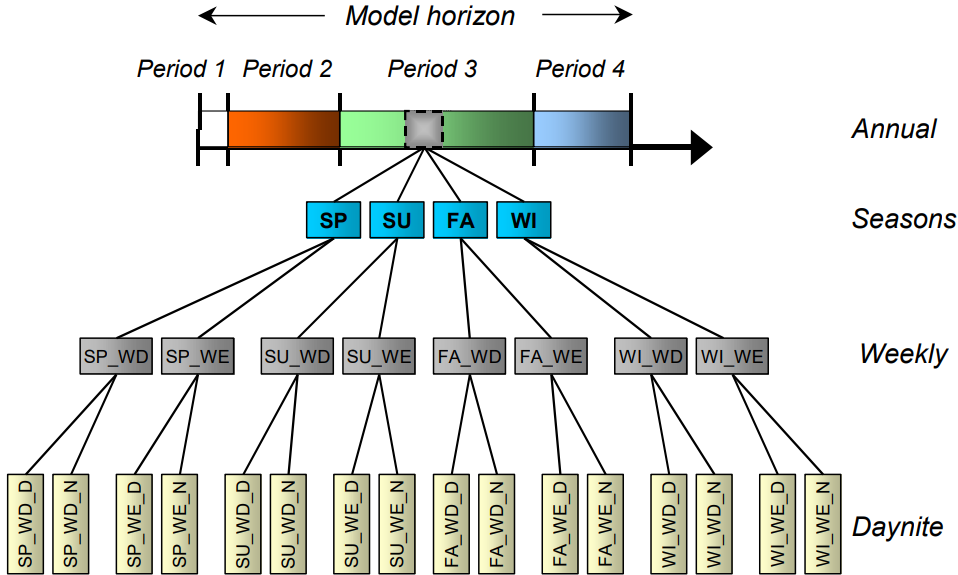
\includegraphics[width=3.2in]{time_horizon.png}
  \caption{Example of a time-slice tree}
  \label{fig1}
  \end{figure}

  \subsection{LEAP}

  LEAP (Long-range Energy Alternatives Planning System) is a energy demand forecasting model developed by the Stockholm Environment Institute (SEI), which is an international research institute that conducts research and provides analysis on environmental and sustainability issues. LEAP is a long-term energy modeling tool that is used to analyze the evolution of energy systems and to evaluate the impacts of different policy scenarios on energy markets, the environment, and economic performance. It is a flexible model that can be used to analyze a wide range of energy systems, including electricity, heat, transport, and industrial systems, and it is designed to be compatible with other models and tools used for energy analysis. The Stockholm Environment Institute (SEI) is a non-profit research institute that conducts research and provides analysis on environmental and sustainability issues to support policy development and decision-making. It has offices and research centers in a number of countries around the world.The structure of LEAP is descripted in Figure xx


  %\subsubsection{Inputs}
  LEAP supports a wide range of different modeling methodologies: on the demand side these range from bottom-up, end-use accounting techniques to top-down macroeconomic modeling. On the supply side, LEAP provides a range of accounting, simulation and optimization methodologies that are powerful enough for modeling electric sector generation and capacity expansion planning, and which are also sufficiently flexible and transparent to allow LEAP to easily incorporate data and results from other more specialized models.

  LEAP operates at two basic conceptual levels. At one level, LEAP's built-in calculations handle all of the "non controversial" energy, emissions and cost-benefit accounting calculations. At the second level, users enter spreadsheet-like expressions that can be used to specify time-varying data or to create a wide variety of sophisticated multi-variable models, thus enabling econometric and simulation approaches to be embedded within LEAP’s overall accounting framework.
 
  %\subsubsection{Time Horizon}
  LEAP  is intended as a medium- to long-term modeling tool. Most of its calculations occur on an annual time-step, and the time horizon can extend for an unlimited number of years. Studies typically include both a historical period known as the Current Accounts, in which the model is run to test its ability to replicate known statistical data, as well as multiple forward looking scenarios. Typically, most studies use a forecast period of between 20 and 50 years.\cite{leap}
  
  \begin{figure}[!t]
  \centering
  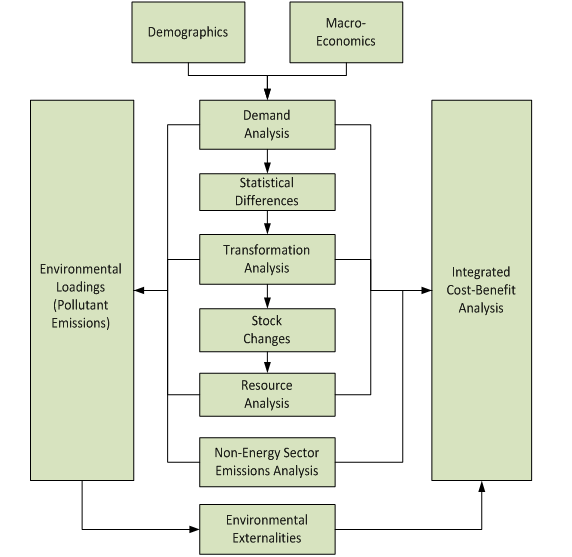
\includegraphics[width=3.2in]{leapstructure.png}
  \caption{The Structure of LEAP's Calculations}
  \label{fig2}
  \end{figure}

  \subsection{PRIMES}
  PRIMES (Policy-supporting Energy Model System) is a large scale applied energy demand forecasting model developed by E3Modelling, a spin-off of the E3MLab at National Technical University of Athens (NTUA). The model is suited for medium-term and long-term (up to 2070) projections in 5-year steps and covers all EU Member States, and EFTA (except Lichtenstein) and candidate countries. It is a Bottom-up Partial equilibrium (PE) model, combines micro-economic foundations of the behavioural modelling with the engineering and energy-system approach, covering all energy sectors and markets at a disaggregated level. The model provides detailed projections of energy demand, supply, prices and investment into the future, covering the entire energy system including emissions. Furthermore, the model captures the technology learning and economies of scale.

  
  The PRIMES model is modular and consists of several sub-models (modules), each one representing the behaviour of a specific agent, a demander or supplier of energy. Sub-models link with each other through a model integration algorithm, which determines equilibrium prices in multiple markets and equilibrium volumes, including cap and trade systems (e.g. ETS), which satisfy balancing and policy, e.g. emissions, constraints and policy targets.

  del captures the technology learning and economies of scale.

  The PRIMES model is modular and consists of several sub-models (modules), each one representing the behaviour of a specific agent, a demander or supplier of energy. Sub-models link with each other through a model integration algorithm, which determines equilibrium prices in multiple markets and equilibrium volumes, including cap and trade systems (e.g. ETS), which satisfy balancing and policy, e.g. emissions, constraints and policy targets.

  PRIMES takes the following as inputs:
  \begin{itemize}
  \item Eurostat and EEA: Energy Balance sheets, Energy prices (complemented by other sources, such IEA), macroeconomic and sectoral activity data (PRIMES sectors correspond to NACE 3-digit classification), population data and projections, physical activity data (complemented by other sources), CHP surveys, CO2 emission factors (sectoral and reference approaches) and EU ETS registry for allocating emissions between ETS and non ETS, Process CO2 emisssions

  \item Technology databases: ODYSSEE-MURE, ICARUS, Eco-design, VGB (power technology costs), TECHPOL – supply sector technologies, NEMS model database, IPPC BAT Technologies

  \item Power Plant Inventory: ESAP SA and PLATTS

  \item RES capacities, potential and availability: JRC ENSPRESO, JRC EMHIRES, RES ninja, ECN, DLR and Observer, IRENA Network infrastructure: ENTSOE, GIE, other operators

  \item Other databases: District heating surveys (e.g. from COGEN), buildings and houses statistics and surveys (various sources, including ENTRANZE project, INSPIRE archive, BPIE), JRC-IDEES, update to the EU Building stock Observatory
  \end{itemize}

  And as for outputs, PRIMES provides, per country represented and for the EU as a whole detailed and comprehensive energy balances of the energy system, related CO2 emissions and detailed economic information associated to the energy system (investments, costs, prices, taxes, ..).\cite{primes}

  \subsection{AIM/ENDUSE}
  AIM/ENDUSE  is a bottom-up technology selection framework for analysis of country-level policies related to greenhouse gas emissions mitigation and local air pollution control, which developed by the National institute for Environmental Studies Japan. Energy and material flows through technology systems in an economy, and consequent emissions, are modeled elaborately. Selection of technologies takes place in a linear optimization framework where system cost is minimized under several constraints like satisfaction of service demands, availability of energy and material supplies, and other system constraints.  The model can perform calculations simultaneously for multiple years. Various scenarios including policy countermeasures can be analyzed in AIM/Enduse. 

  Energy, materials and services can be represented in two ways in the model. An energy or material that is supplied externally to the model is an external energy. Similarly, a service that is demanded externally to the model is an external or final service. Any energy or material that is produced and consumed within the model is an internal service or energy. Service demands are the main external drivers that trigger technology selection decisions based on information on costs. Energy-mix and material-mix are derived from the technology-mix. Finally, emissions of CO2, SO2, and NOx are derived from the information on emission characteristics of energy, materials, and technologies. 

  Outputs of the model include recruited stocks of devices, operating quantities of devices, use of energy-types, level of flow of internal energy or services, emission quantities of CO2, SO2 and NOx, system cost including recruitment costs, operating costs of devices and costs of exchanging removal processes, in each year. These outputs enable evaluation of a particular policy intervention or countermeasure on multiple criteria.\cite{aim}



\section{Summary}
All models above have lots of similarities: On the input side, they all take economic and policy impact into simulation; a time range of several decades are supported. On the output side, 
[mehr Info]


\begin{thebibliography}{1}
  
  \bibitem{UNFCCC}
  UNFCCC. “The Paris Agreement.” United Nations Framework Convention on Climate Change, United Nations, 2016, unfccc.int/process-and-meetings/the-paris-agreement/the-paris-agreement.
  
  \bibitem{srilanka}
  Himanshu AA, Lester CH. Electricity demand for Sri Lanka: a time series analysis. Energy 2008;33:724–39.

  \bibitem{TSA-india}
  Mabel MC, Fernandez E. Growth and future trends of wind energy in India. Renewable and Sustainable Energy Reviews 2008;12:1745–57.

  \bibitem{37}
  B. Liu, J. Nowotarski, T. Hong, and R. Weron, "Probabilistic load forecasting via quantile regression averaging on sister forecasts," IEEETrans. Smart Grid, vol. 8, no. 2, pp. 730–737, Mar. 2017.

  \bibitem{76}
  Y. Wang, N. Zhang, Y. Tan, T. Hong, D. S. Kirschen, and C. Kang, "Combining probabilistic load forecasts," IEEE Trans. Smart Grid, vol. 10, no. 4, pp. 3664–3674, Jul. 2019

  \bibitem{77}
  T. Li, Y. Wang, and N. Zhang, "Combining probability density forecasts for power electrical loads," IEEE Trans. Smart Grid, vol. 11, no. 2, pp. 1679–1690, Mar. 2020.

  \bibitem{9}
  Boßmann, T.; Staffell, I. The shape of future electricity demand: Exploring load curves in 2050s Germany and Britain. Energy 2015, 90, 1317–1333


  \bibitem{time-serie india}
  Kumar U, Jain VK. Time series models (Grey-Markov. Grey Model with rolling mechanism and singular spectrum analysis) to forecast energy consumption in India. Energy 2010; 35(4): 1709–16

  \bibitem{time-serie india ghosh}
  Ghosh, S.: Univariate time-series forecasting of monthly peak demand of electricity in northern India. Int. J. Indian Cult. Bus. Manag. 1(4), 466–474 (2008)

  \bibitem{time-serie Nigeria}
  Mati, A.A., Gajoga, B.G., Jimoh, B., Adegobye, A., Dajab, D.D.: Electricity demand forecasting in Nigeria using time series model. Pac. J. Sci. Technol. 10(2), 479–485 (2009)

  \bibitem{time-serie china}
  Wang, J., Chi, D., Wu, J., Lu, H.Y.: Chaotic time series method combined with particle swarm optimization and trend adjustment for electricity demand forecasting. Expert Syst. Appl. 38(7), 8419–8429 (2011)

  \bibitem{time series clustering}
  Simmhan, Y., Noor, M.U.: Scalable prediction of energy consumption using incremental time series clustering. In: Big Data, IEEE International Conference, pp. 29–36. IEEE (2013)

  \bibitem{O'Neill BC}
  O'Neill BC, Desai M. Accuracy of past projections of US energy consumption. Energy Policy 2005;33(8):979–93.

  \bibitem{Lee CC}
  Lee CC, Chang CP. The impact of energy consumption on economic growth: evidence from linear and nonlinear models in Taiwan. Energy 2007;32(12):2282–94

  \bibitem{Al-Hamadi HM}
  Al-Hamadi HM, Soliman SA. Long-term/mid-term electric load forecasting based on short-term correlation and annual growth. Electrical Power and Energy Systems 2005;74(3):353–61

  \bibitem{Tunc}
  Tunc M, Camdali U, Parmaksizoglu C. Comparison of Turkey's electrical energy consumption and production with some European countries and optimization of future electrical power supply investments in Turkey. Energy Policy 2006;34(1):50–9

  \bibitem{Bessec}
  Bessec M, Fouquau J. The non-linear link between electricity consumption and temperature in Europe: a threshold panel approach. Energy Economics 2008;30(5):2705–21

  \bibitem{Al-Ghandoor A}
  Al-Ghandoor A, Al-Hinti I, Jaber JO, Sawalha SA. Electricity consumption and associated GHG emissions of the Jordanian industrial sector: empirical analysis and future projection. Energy Policy 2008;36(1):258–67.

  \bibitem{Jonsson}
  Jónsson T, Pinson P, Madsen H. On the market impact of wind energy forecasts. Energy Economics 2010;32(2):313–20.

  \bibitem{Utama}
  Utama, N.A., Ishihara, K.N., Tezuka, T., Farzaneh, H., McLellan, B., Zhang, Q.: Energy Demand Forecast for South East Asia Region: an econometric approach with relation to the energy per capita "Curve". In: Zero-Carbon Energy Kyoto 2012, pp. 31–41. Springer, Japan (2013)

  \bibitem{Mtembo}
  Mtembo, V., Taylor, G.A., Ekwue, A.: A novel econometric model for peak demand forecasting. In: Power Engineering Conference (UPEC), 49th International Universities, pp. 1–6. IEEE (2014)


  \bibitem{Dey}
  Dey, H.S., Kabir, M.A., Wadud, Z., Khan, S.I., Azad, M.A.: Econometric modeling and forecasting of natural gas demand for power sector in Bangladesh. In: TENCON 2011–2011 IEEE Region 10 Conference, pp. 1383–1386. IEEE (2011)

  \bibitem{Roming}
  Roming, N., Leimbach, M.: Econometric forecasting of final energy demand using in-sample and out-of-sample model selection criteria (2015)

  \bibitem{Box}
  Box, G.E., Jenkins, G.M., Reinsel, G.C., Ljung, G.M.: Time series analysis: forecasting and control. Wiley, New York (2015)

  \bibitem{Ediger 1}
  Ediger VS, Akar S, Ugurlu B. Forecasting production of fossil fuel sources in Turkey using a comparative regression and ARIMA model. Energy Policy 2006;34(18):3836–46

  \bibitem{Ediger 2}
  Ediger VS, Akar S. ARIMA forecasting of primary energy demand by fuel in Turkey. Energy Policy 2007;35:1701–8.

  \bibitem{Erdogdu}
  Erdogdu E. Natural gas demand in Turkey. Applied Energy 2010;87:211–9

  \bibitem{Conejo}
  Conejo AJ, Plazas MA, Espinola R, Molina AB. Day-ahead electricity price forecasting using the wavelet transform and ARIMA models. IEEE Transactions on Power Systems 2005;20:1035–42.

  \bibitem{Pappas}
  Pappas SS, Ekonomou L, Karamousantas DC, Chatzarakis GE, Katsikas SK, Liatsis P. Electricity demand loads modeling using auto regressive moving average (ARMA) models. Energy 2008;33:1353–60.

  \bibitem{Box 2}
  Box, G. E. P., Jenkins, G. M., \& Reinsel, G. C. (2008). Time series analysis: forecasting and control (4th ed.). Wiley.

  \bibitem{times-docu}
  Loulou, R., Remne, U., Kanudia, A., Lehtila, A., Goldstein, G., 2021. Documentation for the TIMES Model - PART I


  \bibitem{leap}
  Heaps, C.G., 2022. LEAP: The Low Emissions Analysis Platform. [Software version: 2020.1.85] Stockholm Environment Institute. Somerville, MA, USA. https://leap.sei.org

  \bibitem{primes}
  PRIMES MODEL, 2018, \url{https://e3modelling.com/wp-content/uploads/2018/10/The-PRIMES-MODEL-2018.pdf}

  \bibitem{aim}
  Go Hibino1, Rahul Pandey2, Yuzuru Matsuoka3, Mikiko Kainuma4, A Guide to  AIM/Enduse Model, \url{https://www.nies.go.jp/media_kit/16.AIM/Enduse/AIM_Enduse_manual/01_MANUAL_SECTION1.pdf}

\end{thebibliography}

\end{document}


